\documentclass{article}
\usepackage[utf8]{inputenc}
\usepackage{graphicx}% http://ctan.org/pkg/graphicx

\usepackage{amsmath}
\usepackage{amsfonts}

\usepackage[top=2cm,bottom=2.5cm,left=3cm,right=3cm]{geometry}
\usepackage[font=small,labelfont=bf]{caption}

\usepackage{enumitem}
\usepackage{listings}
\usepackage{courier}
\lstset{basicstyle=\footnotesize\ttfamily,breaklines=true}

\usepackage{hyperref}
\usepackage{xcolor}
\hypersetup{
    colorlinks,
    linkcolor={red!50!black},
    citecolor={blue!50!black},
    urlcolor={blue!66!green}
}

\begin{document}

\title{\href{https://tiborstanko.sk/teaching/geo-num-2016/tp1.html}{TP1 : Bézier curves, De Casteljau's algorithm}}\label{tp1-buxe9zier-curves-de-casteljaus-algorithm}
\date{February 5, 2016}
\author{Tibor Stanko}
\maketitle

\section{Bézier curves}\label{buxe9zier-curves}

A degree \(n\)
\href{https://en.wikipedia.org/wiki/B\%C3\%A9zier_curve}{Bézier curve}
takes the form

\[
\mathbf x(t) = \sum_{i=0}^{n} \mathbf b_i B_i^n(t) \qquad t \in [0,1]
\]

where

\[
B_{i}^{n}(t) = \begin{pmatrix}n \\ i\end{pmatrix} (1-t)^{n-i} t^i
\]

are the degree \(n\)
\href{https://en.wikipedia.org/wiki/Bernstein_polynomial}{Bernstein
polynomials}, and the binomial coefficients are defined as

\[
\begin{pmatrix}n \\ i\end{pmatrix} = \frac{n!}{(n-i)! i!}.
\]

The Bézier points \(\mathbf b_i \in \mathbb R^d\) form the \emph{control
polygon}.

\section{De Casteljau's algorithm}\label{de-casteljaus-algorithm}

\begin{itemize}
\itemsep1pt\parskip0pt\parsep0pt
\item
  input: Bézier points \(\mathbf b_i\) for \(i = 0, \dots, n\), and
  parameter \(t \in [0,1]\).
\item
  output: The point \(\mathbf b_0^n\) on the curve.
\item
  set \(\mathbf b_i^0 = \mathbf b_i\) and compute the points
\end{itemize}
\[
\mathbf b_i^k (t) = (1-t) \mathbf b_i^{k-1} + t \mathbf b_{i+1}^{k-1} \qquad \text{for} \qquad k=1,\dots,n, \quad i=0,\dots,n-k.
\]

\begin{figure}[htb]
\centering
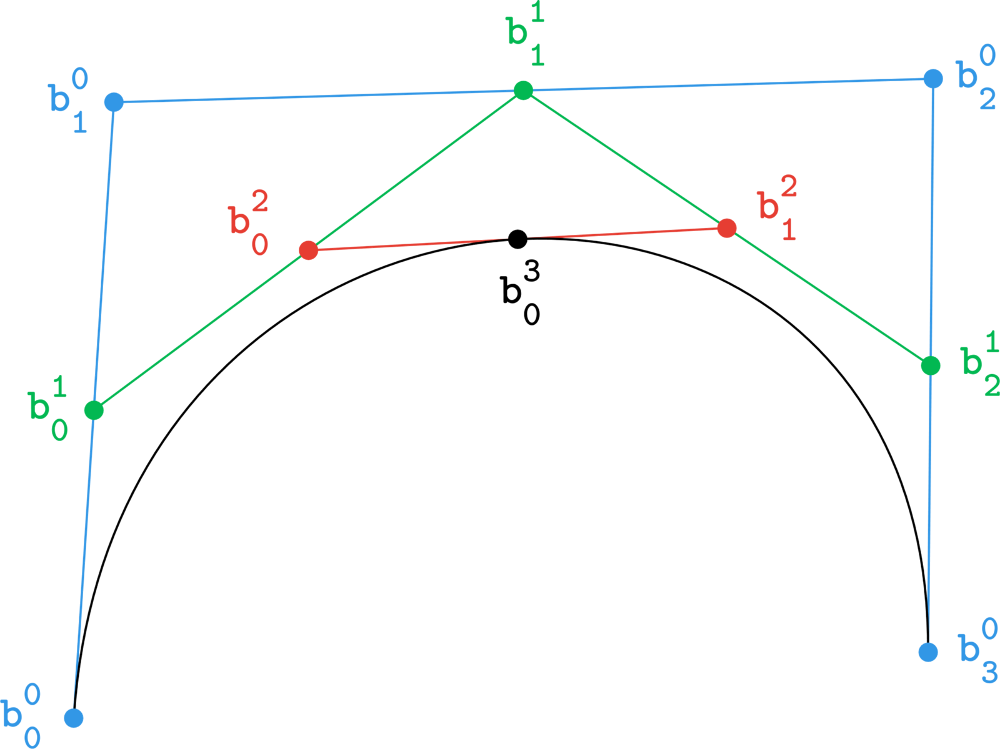
\includegraphics[width=0.8\textwidth]{../assets/geo-num-2016/casteljau-curve.png}
\caption{Visualisation of the steps of the De Casteljau's algorithm.}
\end{figure}

The \href{https://en.wikipedia.org/wiki/De_Casteljau\%27s_algorithm}{De
Casteljau's algorithm} provides an efficient means for evaluating a
Bézier curve \(\mathbf{x}(t)\).
It is useful to look at this algorithm in its schematic form.
For a quartic curve (\(n=4\)):

\[
\begin{array}{ccccccccc}
\mathbf b_0 = \mathbf b_0^0 &        &               &        &               &        &               &        & \\
                            & \ddots &               &        &               &        &               &        & \\
\mathbf b_1 = \mathbf b_1^0 & \dots  & \mathbf b_0^1 &        &               &        &               &        & \\
                            & \ddots &               & \ddots &               &        &               &        & \\
\mathbf b_2 = \mathbf b_2^0 & \dots  & \mathbf b_1^1 & \dots  & \mathbf b_0^2 &        &               &        & \\
                            & \ddots &               & \ddots &               & \ddots &               &        & \\
\mathbf b_3 = \mathbf b_3^0 & \dots  & \mathbf b_2^1 & \dots  & \mathbf b_1^2 & \dots  & \mathbf b_0^3 &        & \\
                            & \ddots &               & \ddots &               & \ddots &               & \ddots & \\
\mathbf b_4 = \mathbf b_4^0 & \dots  & \mathbf b_3^1 & \dots  & \mathbf b_2^2 & \dots  & \mathbf b_1^3 & \dots  & \mathbf b_0^4 = \mathbf x(t) 
\end{array}
\]

\section{Code}\label{code}
\begin{lstlisting}
git clone https://github.com/bbrrck/geo-num-2016.git
cd geo-num-2016/TP1
mkdir build
cd build
cmake ..
make ./geonum_TP1
\end{lstlisting}
For rendering, you can use gnuplot or matplotlib.
While still in the \texttt{build/} directory, test them by running
\begin{lstlisting}
gnuplot -p ../plots/plot.gnu
python ../plots/plot.py
\end{lstlisting}
Many of you have reported problems with gnuplot due to the line set
terminal qt. Change it to something else to make things work, e.g. set
terminal x11. For a complete list of terminals available on your
machine, execute 
\begin{lstlisting}
echo 'set terminal' | gnuplot
\end{lstlisting}

\section{ToDo}\label{todo}

\begin{enumerate}
\def\labelenumi{\arabic{enumi}.}
\item
  Implement the computation of a curve point \(\mathbf x(t)\) using
  Bernstein polynomials.
\item
  Implement the De Casteljau algorithm for a parameter \(t\).
\item
  Evaluate the curve using both methods and compare their performance
  the De Casteljau algorithm for various sampling densities.
\item
  Visualise the curve and its Bézier polygon. Use all input files from
  the data/ folder.
\item
  Visualise the intermediate polygons \(\mathbf b_i^k\) from the De
  Casteljau algorithm for a fixed parameter \(t\). (Only the simple.bcv
  is enough.)
\end{enumerate}

\section{Resources}\label{resources}

\begin{itemize}
\itemsep1pt\parskip0pt\parsep0pt
\item
  \href{http://www.sciencedirect.com/science/book/9780444511041}{Handbook
  of CAGD}, edited by Gerald Farin, Josef Hoschek, Myung-Soo Kim
\item
  \href{http://pomax.github.io/bezierinfo/}{A Primer on Bézier Curves}
  by Pomax
\item
  \href{http://jeremykun.com/2013/05/11/bezier-curves-and-picasso/}{Bézier
  Curves and Picasso} by Jeremy Kun
\item
  \href{http://learn.scannerlicker.net/2014/04/16/bezier-curves-and-type-design-a-tutorial/}{Bézier
  Curves and Type Design: A Tutorial} by Fábio Duarte Martins
\item
  \href{http://bezier.method.ac/}{The Bézier Game}
\item
  \href{http://tholman.com/bezier-curve-simulation/}{Bézier Curve
  Simulation}
\end{itemize}

\end{document}